\newpage
\section{Hardware implemented blocks}

This section will describe components that were implemented on the FPGA of RaMstix board - encoders, PWMs, and GPMC interface. The latter has been discussed previously and for the sake of clarity in the report will not be repeated here.

\subsection{Encoder}
As it was requested in the original instructions for the project and since encoders were to be operated over the GPIO pins of the boards available, hardware implementation was the obvious choice. By definition, encoders generate two waveforms - named A and B. These waveforms are in quadrature of each other - by counting the pulses and determining phase offset we can calculate the relative position. Example waveforms can be found in the figure \ref{encoder_waves} below.\\

\begin{figure}[!ht]
\centering
 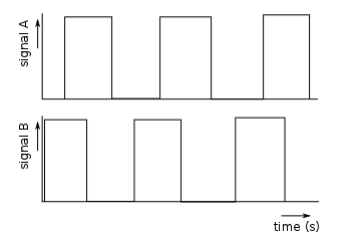
\includegraphics[width=0.7\textwidth]{images/encoder.png}
 \caption{Example waveforms generated by the encoders}
 \label{encoder_waves}
\end{figure}

Using this example, we can determine that waveform B is leading A - meaning that position should be decremented. The amount by which it will be decremented is calculated by counting pulses of A and B. In our implementation, a rotation is defined as a sequence of A and B in the following manner - [11], [10], [00], [01], [11]. This would correspond to decreasing position by 1 unit, while [11], [01], [00], [10], [11] would indicate that position should be incremented. First position is taken as "0" and can change within the range signed 8-bit number - from -128 to 127. Encoder has been implemented as an asynchronous hardware unit. While the FPGA system clock is set at 50MHz, which is sufficiently high for sampling values from the encoder in order not to lose anything, it was a design choice to make it operate based on the input from the encoder itself. Therefore, in its final form, our encoder block would not execute any calculations if there is no rotation.\\

Additionally, encoder block has been given an "enable" and a "reset" input. If reset signal is asserted by the master, position would be set back to 0. In order to operate this block, enable signal has to be set to "1".

There are two instances of this component, each corresponding to one of the two encoders used in the JIWY2 setup - one for tilt and one for pan movements.

 
\begin{table*}[!htbp]
\small
   \caption{Signal description of VHDL implementation of the encoder block}
   \centering
%\renewcommand\arraystretch{1.5}
\begin{tabular}{l l l l} \hline\\ 
\textbf{Signal Name} & \textbf{I/O} & \textbf{Data Type} & \textbf{Description}  \\ \hline
reset\_n & Input  & std\_logic & Reset input \\ \hline
position & Output  & std\_logic\_vector & Calculated 8-bit position for output  \\ \hline
enable & Input & std\_logic & Enable signal \\ \hline
enc\_in & Output & std\_logic\_vector & 2-bit input, format: A\&B \\ \hline
\end{tabular}
\vspace{-0.5cm}
\end{table*}

\subsection{Pulse width modulation}
Pulse width modulation is used to control the speed of the motors, as well as their direction. In order to do this, an H-bridge was provided in the system. From the datasheet of this H-bridge, we were able to determine which signals are required for proper operation of the motors.\\

This block is generating three output signals - A, B, and C. First two signals are used to encode the direction of rotation - clockwise or counterclockwise. The last signal, C, is a square wave, controlling duty cycle of which determines how fast the motors will spin. The frequency for this wave could be variable, but by the recommendations from the instructions it was chosen to be 20KHz (however, the possibility to change this later if needed was implemented anyway). Since waveform generation is involved, this block needs to be synchronous to the 50MHz system clock. Reset is set as asynchronous, active high.\\

There 4 modes of operation, based on the specification. These modes are controlled by a configurable 2-bit input port, labeled "direction".
\begin{enumerate}
 \item Clockwise rotation: AB = [10]; direction = [00]
 \item Counterclockwise rotation: AB = [01]; direction = [01]
 \item Brake to Vcc: AB = [11]; direction = [10]
 \item Brake to GND: AB = [00]; direction = [11]
\end{enumerate}

Generation of a PWM signal is rather straightforward - implementation is based on a counter. Until the counter is less and not equal to the value specified by the duty cycle port, output signal C is set to "1". The rest of the time, until counter is not equal to the value specified by the period, C is set to "0". Period is limited from 25Hz to 20KHz and our system clock is more than fast enough for this. In hardware, this is represented as an integer in range of 0 to 2000000 Reset signal asserted will trigger a reset state and A&B signals will be set to "0" (corresponding to braking to GND), setting the counter to 0 and output PWM signal to 0 as well. Enable signal is included in this block as well and performs its obvious function - enabling or disabling the outputs.

\begin{table*}[!htbp]
\small
   \caption{Signal description of VHDL implementation of the PWM block}
   \centering
%\renewcommand\arraystretch{1.5}
\begin{tabular}{l l l l} \hline\\ 
\textbf{Signal Name} & \textbf{I/O} & \textbf{Data Type} & \textbf{Description}  \\ \hline
reset\_n & Input  & std\_logic & Reset input \\ \hline
CLOCK\_50 & Input  & std\_logic & Clock input \\ \hline
enable & Input & std\_logic & Enable signal \\ \hline
direction & Input & std\_logic\_vector & 2-bit input for direction \\ \hline
PWM\_PERIOD & Input & integer & PWM period \\ \hline
PWM\_DUTY & Input & integer & PWM duty cycle \\ \hline
IN\_A & Output & std\_logic & A signal output \\ \hline
IN\_B & Output & std\_logic & B signal output \\ \hline
PWM\_C & Output & std\_logic & PWM signal output \\ \hline
\end{tabular}
\vspace{-0.5cm}
\end{table*}

\subsection{Overview of the hardware implementation}
The development process for our project was done in parallel and therefore verification and testing of the aforementioned blocks was done separately first. Main limiting factors of the full hardware implementation in that case are programming/reprogramming speed and limited flexibility. It is assumed as common sense that a hardware block cannot be configured on the fly once it has been routed and placed on the FPGA. For this reason, it is obvious that software control will help and speed up our design process. NIOS II softcore processor is a powerful tool in that sense, as it allows us to enable/disable, reset, write to and read values from the encoder and PWM blocks very quickly. Using a JTAG UART core we are able to display values monitored in the console on the development PC and immediately determine if the functionality is correct and as expected. Below, a section of a program written to control the encoder block is included:

\begin{lstlisting}[language=C]
while(i<200){
	IOWR(ESL_BUS_DEMO_0_BASE, 0x00, 1 << 31 | 0x03); //11
	usleep (1500000);
	nReadOut = IORD(ESL_BUS_DEMO_0_BASE, 0x00);
	printf ("after 0x03: %d", nReadOut);
	IOWR(ESL_BUS_DEMO_0_BASE, 0x00, 1 << 31 | 0x02); //10
	usleep (2500000);
	nReadOut = IORD(ESL_BUS_DEMO_0_BASE, 0x00);
	printf ("after 0x02: %d", nReadOut);
	IOWR(ESL_BUS_DEMO_0_BASE, 0x00, 1 << 31 | 0x00); //00
	usleep (2500000);
	nReadOut = IORD(ESL_BUS_DEMO_0_BASE, 0x00);
	printf ("after 0x00: %d", nReadOut);
	IOWR(ESL_BUS_DEMO_0_BASE, 0x00, 1 << 31 | 0x01); //01
	usleep (1500000);
	nReadOut = IORD(ESL_BUS_DEMO_0_BASE, 0x00);
	printf ("after 0x01: %d", nReadOut);
	i++;
}
\end{lstlisting}

This loop will be repeated 200 times, simulating an input from the real encoder and its outputs A&B. IOWR() performs a write to the input register of the encoder, located at the base address. NIOS II uses 32-bit registers and the MSB is used as the "enable" bit, while two LSBs are the considered to be inputs. IORD() performs a read from the base address of the encoder, giving us the position it has calculated. This read is performed after each write, in order to ensure that we do not wrongfully increment or decrement the position. Later, the system was directly connected to physical setup, and only read operations were executed, while camera was moved manually and the change in position was observed in the console output. A similar approach was used for the PWM block too.\\

After it was confirmed that both blocks are performing as expected with the real setup, we had to decide whether to keep using the NIOS based system or not. The following points were considered:

\begin{enumerate}
 \item Communication protocol used - \textit{GPMC}
 \item Hardware implementation for the protocol available - \textit{Yes}
 \item Availability to map ports of the hardware blocks to the communication registers - \textit{Yes}
 \item Need for further tuning of the hardware platform - \textit{No. In an unforeseen case, the change is expected to be easily implemented in VHDL}
 \item Time for compilation and programming of the FPGA without NIOS - \textit{Reduced (with respect to including NIOS)}
\end{enumerate}

It shall be seen that most of these points allude to using a full hardware system on the FPGA, without any softcore included. It shall also be seen that despite this decision, the system remains fully software configurable. All ports of our HW blocks are mapped to the registers used by GPMC (even reset and enable), therefore allowing us to exhibit behaviour similar to what we had in NIOS initially. During the implementation phase of GPMC, software to perform necessary tasks was written as part of the assignments, and therefore this shift did not cost us any development time either.\\

Subjectively, in our opinion, elimination of NIOS II actually saves us time and makes our system more reliable and predictable. In our experience, Eclipse IDE that is required in order to operate with NIOS II is extremely unstable, with issues such as unexpected crashes, bugs, and other unwanted conditions. While these situations are not very common, but occur frequent enough to be noted, the main issue lies in the connectivity to the FPGA board. After programming the FPGA with the synthesized VHDL, Eclipse has to establish a connection to the NIOS II running on the FPGA. Unfortunately, we have encountered an issue where this connection could not established, despite multiple attempts, with different configurations, and assistance from the teaching staff of the course. This, if not the main, was definitely playing a key role in the choice of fully hardware system over integration with NIOS II. Since the lab hours with access to the physical setup were limited, these issues were out of scope for "at-home" development and testing, and could not be reproduced with simulations, costing us invaluable time that could be used for tuning our design on the actual physical setup.

\newpage
\section{Conclusion}

In the end, we have been successful to implement a demonstration project, where camera was able to track an object of our choice, with the movements smooth and precise enough. In fact, our choice of control loop implementation is not obvious unless we tell the observer that included and proposed 20-sim model was not utilized.\\

Overall, we have been mostly using our previous knowledge and skills in order to complete the assignments throughout this course. Issues that arose during this process were solved with the help of searching and reading manuals and tutorials online, and in the extreme cases by involving the teaching assistants. These cases were only related to the times that the actual physical setup was incorrect, due to other teams changing, disassembling, or even assembling it back incorrectly, hopefully unknowingly. If possible, it would be better and more beneficial if some instructions were defined and declared at the start of the course in a more clear manner. We have often found ourselves struggling with connecting to the platforms, due to missing or incorrect instructions, or other factors outside of our control. This has resulted in significant delays or lost time during the limited lab hours. While it may be an interesting experience to debug and fix errors of a given and default design (such as GPMC software addressing example), we do not have time left for debugging our own functions (as we cannot do that before we have loaded our designs on the boards). In addition, it would be a nice idea to include some verified simple tests (with or withour source codes), that would help us to check whether the physical setup is broken or it is our design that needs to be checked.\\

All things considered, this is was an interesting project to work on, and hopefully once the issues are addressed, it will be even more enjoyable.